%%This work may be distributed and/or modified under the conditions of the LaTeX Project Public License, either version 1.3 of this license or (at your option) any later version.
%--------------------------------------------------------------

% TEMPLATE PARA TRABALHO DE CONCLUSÃO DE CURSO
% Universidade Tecnológica Federal do Paraná - UTFPR
% Disponibilizado e mantido pelo LAMIA - Laboratório de Aprendizado de Máquina e Images Aplicados à Indústria
% lamia-sh@utfpr.edu.br - naves@utfpr.edu.br
% Campus Santa Helena
% Bacharelado em Ciência da Computação
% Customização da classe abnTeX2 (http://www.abntex.net.br/) para as normas da UTFPR - SH
% LaTeX:  abnTeX2   
% Projeto hospedado em: <https://github.com/lamiautfpr/TCC-Latex-COCIC-UTFPR-SH>
% Autor: Thiago França Naves

\documentclass{lamia-tcc-utfpr-sh}

%%%%%%%%%%%%%%%%%%%%%%%%%%%%%%%%%%%%%%%%%%%%%%%%%%%%%%%%%%%%
%P A C O T E S
%%%%%%%%%%%%%%%%%%%%%%%%%%%%%%%%%%%%%%%%%%%%%%%%%%%%%%%%%%%%
% Adicione aqui seus pacotes

\usepackage{csquotes} %pacote com comandos para fazer citações de longos textos ou parágrafos de alguma referência

%pacote com todas as funções de bibliograficas modernas do latex, pesquise as variações do comando \cite disponíveis com o biblatex  
\usepackage[
	backend=biber, 
	style=abnt, 
	uniquename=mininit, 
	giveninits, % Abrevia os primeiros nomes da bibliografia 
	extrayear, % Diferencia os nomes com letras (bibliografia e referencia)
	repeatfields, % Imprime campos repetidos na bibliografia. O padrão desse pacote é substituílos por traços sublineares. Contudo, a UTFPR prefere os campos repetidos.
	backref=false, % Desabilita a referencia da página onde foi citado.
	noslsn % As abreviações [s.l], [s.n] e [s.l.: s.n.] são ocultadas. Essas abreviações são permitidas pela norma NBR 6023:2018, porém o UTFPR-SH prefere não utilizá-los.

]{biblatex} 

\addbibresource{elementos-postextuais/referencias.bib} %endereço do seu arquivo com as referências bibliográficas
\hypersetup{
    colorlinks=true,       		% Se não quiser cores no texto marcar como false
    	linkcolor=black,          	% cor dos links do texto como o sumário
    	citecolor=blue,        		% cor das citações no texto
    	filecolor=magenta,      	% cor de arquivos externos 
		urlcolor=blue,}             % cor de url no texto e nas referências bibliográficas
		
%%%%%%%%%%%%%%%%%%%%%%%%%%%%%%%%%%%%%%%%%%%%%%%%%%%%%%%%%%%%
%I N I C I O  D O  D O C U M E N T O
%%%%%%%%%%%%%%%%%%%%%%%%%%%%%%%%%%%%%%%%%%%%%%%%%%%%%%%%%%%%
\begin{document}

% título da monografia é obrigatório
\title{\textbf{Título da monografia}}

% autor é obrigatório; máximo de 3 autores (se TCC Empresa)
\author{Nome completo }{Certamente estes parágrafos não irão atender a todas as pessoas que fizeram parte dessa importante fase de minha vida. Portanto, desde já peço desculpas àquelas que não estão presentes entre essas palavras, mas elas podem estar certas que fazem parte do meu pensamento e de minha gratidão. 

Agradeço ao meu orientador Prof. Dr. Fulano, pela sabedoria com que me guiou nesta trajetória.

Aos meus colegas de sala.

A Secretaria do Curso, pela cooperação.

Gostaria de deixar registrado também, o meu reconhecimento à minha família, pois acredito que sem o apoio deles seria muito difícil vencer esse desafio. 

\textcolor{red}{Se o aluno recebeu bolsa de fomento à pesquisa, informar o nome completo da agência de fomento. Ex: Capes, CNPq, Fundação Araucária, etc.}

Enfim, a todos os que por algum motivo contribuíram para a realização desta pesquisa.

\textcolor{red}{Atenção: não utilizar este exemplo na versão final. Use a sua criatividade!}
}
%\author{Nome completo aluno 2}{Certamente estes parágrafos não irão atender a todas as pessoas que fizeram parte dessa importante fase de minha vida. Portanto, desde já peço desculpas àquelas que não estão presentes entre essas palavras, mas elas podem estar certas que fazem parte do meu pensamento e de minha gratidão. 

Agradeço ao meu orientador Prof. Dr. Fulano, pela sabedoria com que me guiou nesta trajetória.

Aos meus colegas de sala.

A Secretaria do Curso, pela cooperação.

Gostaria de deixar registrado também, o meu reconhecimento à minha família, pois acredito que sem o apoio deles seria muito difícil vencer esse desafio. 

\textcolor{red}{Se o aluno recebeu bolsa de fomento à pesquisa, informar o nome completo da agência de fomento. Ex: Capes, CNPq, Fundação Araucária, etc.}

Enfim, a todos os que por algum motivo contribuíram para a realização desta pesquisa.

\textcolor{red}{Atenção: não utilizar este exemplo na versão final. Use a sua criatividade!}
}
%\author{Nome completo aluno 3}{Certamente estes parágrafos não irão atender a todas as pessoas que fizeram parte dessa importante fase de minha vida. Portanto, desde já peço desculpas àquelas que não estão presentes entre essas palavras, mas elas podem estar certas que fazem parte do meu pensamento e de minha gratidão. 

Agradeço ao meu orientador Prof. Dr. Fulano, pela sabedoria com que me guiou nesta trajetória.

Aos meus colegas de sala.

A Secretaria do Curso, pela cooperação.

Gostaria de deixar registrado também, o meu reconhecimento à minha família, pois acredito que sem o apoio deles seria muito difícil vencer esse desafio. 

\textcolor{red}{Se o aluno recebeu bolsa de fomento à pesquisa, informar o nome completo da agência de fomento. Ex: Capes, CNPq, Fundação Araucária, etc.}

Enfim, a todos os que por algum motivo contribuíram para a realização desta pesquisa.

\textcolor{red}{Atenção: não utilizar este exemplo na versão final. Use a sua criatividade!}
}

% orientador é obrigatório
\advisor[Prof.]{Prof. Me. ou Dr. Xxx}{}

% co-orientador é opcional
%\coadvisor[Prof.]{Nome do co-orientador,~M.Sc.}{}

% máximo de 3 integrantes da banca (orientador e co-orientador já são adicionados automaticamente)
\banca[Prof.]{Nome do participante banca 1,~D.Sc.}{}
\banca[Prof.]{Nome do participante banca 2,~D.Sc.}{}

\location{Santa~Helena}{PR}{Brasil}

% mês e ano de defesa
\date{Junho}{2019}
\maketitle

% Hifenização de palavras que não estão no dicionário, coloque aquelas necessárias do seu texto
\hyphenation{%
	qua-dros-cha-ve
	Kat-sa-gge-los
}

\startdocument

%%%%%%%%%%%%%%%%%%%%%%%%%%%%%%%%%%%%%%%%%%%%%%%%%%%%%%%%%%%%
% D E D I C A T O R I A (opcional)
%%%%%%%%%%%%%%%%%%%%%%%%%%%%%%%%%%%%%%%%%%%%%%%%%%%%%%%%%%%% 
\makededicationpage

%%%%%%%%%%%%%%%%%%%%%%%%%%%%%%%%%%%%%%%%%%%%%%%%%%%%%%%%%%%%
% A G R A D E C I M E N T O S
%%%%%%%%%%%%%%%%%%%%%%%%%%%%%%%%%%%%%%%%%%%%%%%%%%%%%%%%%%%% 
\makethankspage

%%%%%%%%%%%%%%%%%%%%%%%%%%%%%%%%%%%%%%%%%%%%%%%%%%%%%%%%%%%%
% E P I G R A F E (opcional)
%%%%%%%%%%%%%%%%%%%%%%%%%%%%%%%%%%%%%%%%%%%%%%%%%%%%%%%%%%%% 
\makeepigraphpage

%%%%%%%%%%%%%%%%%%%%%%%%%%%%%%%%%%%%%%%%%%%%%%%%%%%%%%%%%%%%
% R E S U M O
%%%%%%%%%%%%%%%%%%%%%%%%%%%%%%%%%%%%%%%%%%%%%%%%%%%%%%%%%%%%
\begin{abstract}{
  SOBRENOME, Prenome do Autor. Título do trabalho: subtítulo. Ano de defesa. 50f. (total de folhas). Trabalho de Conclusão de Curso (Bacharelado em Ciência da Computação) – Universidade Tecnológica Federal do Paraná. Santa Helena. 

O resumo deve conter no máximo 500 palavras. Não deve conter citações. Deve ser redigido em parágrafo único, espaçamento simples e seguido de 3 a 5 palavras representativas do conteúdo do estudo (palavras-chave). Usar o verbo na terceira pessoa do singular, com linguagem impessoal (pronome SE), e preferencialmente voz verbal ativa. Inserir o objetivo do trabalho, e descrever brevemente a metodologia adotada, os resultados obtidos e a conclusão (se houver).

Para definir as palavras-chave (e suas correspondentes em inglês no abstract) consultar em Termo tópico do Catálogo de Autoridades da Biblioteca Nacional, disponível em: \url{http://acervo.bn.br/sophia_web/index.html} [avaliar se essa informação procede para Ciência da Computação]

}
\bigskip
% Palavras-chave separadas por ponto
\palavraschave{Palavrachave1. Palavrachave2. Palavrachave3. Palavrachave4. Palavrachave5}
\end{abstract}

%%%%%%%%%%%%%%%%%%%%%%%%%%%%%%%%%%%%%%%%%%%%%%%%%%%%%%%%%%%%
% A B S T R A C T
%%%%%%%%%%%%%%%%%%%%%%%%%%%%%%%%%%%%%%%%%%%%%%%%%%%%%%%%%%%%
\begin{englishabstract}{
  SOBRENOME, Prenome do Autor do Trabalho. Title of the working: subtitle. Ano de defe-sa. 101p. Work of Conclusion Course (Graduation in Computer Science) – Federal Technol-ogyUniversity – Paraná. Santa Helena. 

Versão do resumo em português para o idioma de divulgação internacional, que é a língua inglesa. 


}
\bigskip
% Palavras-chave separadas por ponto
\keywords{Keyword1. Keyword2. Keyword3. Keyword4. Keyword5}
\end{englishabstract}

%%%%%%%%%%%%%%%%%%%%%%%%%%%%%%%%%%%%%%%%%%%%%%%%%%%%%%%%%%%%
% L I S T A S
%%%%%%%%%%%%%%%%%%%%%%%%%%%%%%%%%%%%%%%%%%%%%%%%%%%%%%%%%%%%
% Figuras (opcional)
\makefigurespage

% Tabelas (opcional)
\maketablespage

% Algoritmos
%\makelistingspage

% Abreviaturas (devem estar em ordem alfabética)
\makeabrevpage{\item [BPS] bits por segundo
\item [CGI] Common Gateway Interface (Interface de Porta Comum)
\item [SRAM] Static Random-Access Memory
\item [EEPROM]  Electrically Erasable Programmable Read-Only Memory


}

% Símbolos (devem estar em ordem alfabética)
\makesymbolspage{\item [$\bar{X}$] Tempo médio de uma amostra
\item [$\sigma$] Desvio-padrão
\item [\textit{n}] Número de valores da amostra
\item [$\Delta$] Variação do intervalo de confiança de 95% para a estimação da média da população
}

% Sumário 
\maketocpage

%%%%%%%%%%%%%%%%%%%%%%%%%%%%%%%%%%%%%%%%%%%%%%%%%%%%%%%%%%%%
% C O N T E Ú D O - T E X T O
%%%%%%%%%%%%%%%%%%%%%%%%%%%%%%%%%%%%%%%%%%%%%%%%%%%%%%%%%%%%
\startcontent
\chapter{INTRODUÇÃO}\label{chp:INTRODUCAO}

Parte inicial do texto, na qual devem constar o tema e a delimitação do assunto tratado, objetivos da pesquisa e outros elementos necessários para situar o tema do trabalho. Após o início de uma seção, recomenda-se a inserção de um texto ou, no mínimo, uma nota explicativa sobre a seção iniciada. Evitar, por exemplo, figura \ref{fig:WhatNotToDo}:

\begin{figure}[htb]
	\centering
	\caption{Exemplo do que não é recomendado.}
	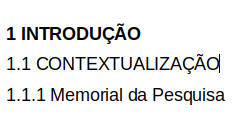
\includegraphics[scale=0.6]{imagens/what-not-to-do.png} 
	\newline {\footnotesize \textbf{Fonte: Autoria própria.}}
	\label{fig:WhatNotToDo}
\end{figure}

\section{OBJETIVOS}\label{sec:OBJETIVOS}
Expõem-se a seguir os objetivos geral e específicos que se pretende atingir com o trabalho . Ver mais exemplos no Anexo 1. 

\subsection{Geral}\label{sec:Geral}
Desenvolver um sistema de Internet of Things (IoT) automatizado que controle a entrada e saída de pessoas em áreas de acesso restrito, identifique suas funções institucionais por meio da tecnologia RFID, e registre o acesso via portas com trava ou catraca.


\subsection{Específicos}\label{sec:Especificos}
\begin{enumerate}
	\item Estudar conceitos básicos relativos a controle de acesso orientado a contextos; 
	
	\item Fazer uma proposta inicial de ambiente;
	
	\item Implementar um protótipo;
	
	\item Desenvolver um módulo Web para controle por parte do administrador, que permita monitorar os registros e gerenciar permissões
\end{enumerate}


\section{CONTRIBUIÇÕES DO TRABALHO}\label{sec:CONTRIBUICOES}
Explicitar as contribuições do trabalho para a sociedade, ou seja, sua pertinência. Por exemplo, no desenvolvimento de um sistema de controle com IoT, a contribuição é o ganho que um sistema desses pode trazer à área de organização escolar, uma vez que automatiza por completo as tarefas, junto com uso eficiente de TFID aliado a um sistema de controle funcional pela Web. Com essas características, o sistema apresenta melhorias em relação ao controle tradicional feito nesses ambientes e supera outras abordagens que não consideram as automatizações aqui propostas. [verificar enumeração]


\section{JUSTIFICATIVA}\label{sec:JUSTIFICATIVA}
A justificativa refere-se a por que é importante e válida a realização do trabalho. Trata-se de convencer o leitor de que o trabalho de pesquisa  apresenta contribuições específicas para a Ciência da Computação. Deve exaltar a importância da pesquisa e a relação de outras pesquisas sobre os mesmos assuntos. [adaptar texto para diferenciar do \ref{sec:CONTRIBUICOES}, colocar exemplo aqui e diretriz no comentário].


\section{DELIMITAÇÕES DO TRABALHO}\label{sec:DELIMITACOES}
Identificar e justificar aqui as delimitações do trabalho em relação a sua construção e objetivos a ser alcançados. Limitações podem estar presentes na: forma como os experimentos foram conduzidos, por falta de, por exemplo, equipamento específico, software ou recursos em geral; forma como a metodologia foi estabelecida, ignorando alguma etapa que por ventura existe, mas não será abordada devido ao viés do trabalho; ou em características gerais do trabalho, em que alguma limitação foi imposta para adequação à construção do trabalho e satisfação dos objetivos principais. [escopo, exemplo]

\chapter{REVISÃO DA LITERATURA}\label{chp:REVISAO}

O desenvolvimento do trabalho é composto por 3 seções: Revisão da Literatura (ou Referencial Teórico); Metodologia; e Análise dos Resultados, e pode conter outras além dessas. A revisão da literatura deve ser apresentada em forma de texto e seu conteúdo demonstra conhecimento da literatura científica sobre o tema do trabalho. O texto pode ser dividido, para fins didáticos, em subseções. Esta seção é permeada de autores, é o local em que há mais intertextualidade no trabalho. Assim, inclui basicamente citações indiretas (paráfrases) e diretas (curtas e longas). Aqui, o autor explicita a contribuição de outros campos do conhecimento que são envolvidos na pesquisa e outras pesquisas relacionadas ao tema, as conclusões que esses autores chegaram, o que é consenso, as discordâncias entre autores. 


\section{INTERTEXTUALIDADE}\label{sec:INTERTEXTUALIDADE}
No referencial teórico e em outras seções em que a intertextualidade é necessária, devem-se citar trabalhos clássicos, mas priorizar trabalhos dos últimos 10 anos. Podem-se usar artigos científicos, livros, TCCs, dissertações, teses, monografias e sites oficiais. Não são permitidos textos jornalísticos, Wikipédia e de blogues. É importante a utilização de referências em inglês no trabalho, livros e principalmente artigos de revista. O banco do IEEE é uma boa sugestão de fonte de pesquisa nessa língua. 

Devem-se seguir as normas da Associação Brasileira de Normas Técnicas (ABNT)  NBR 10520, Informação e documentação – Citações em documentos – Apresentação,  para fazer a intertextualidade por referenciação. 

\section{ESTADO DA ARTE}\label{sec:ESTADOARTE}

No referencial teórico deve haver uma subseção para o estado da arte, em que se apresenta uma busca de anterioridade sobre o produto a ser desenvolvido, por exemplo, um software ou hardware, uma metodologia, bem como as publicações mais atuais e conceituadas sobre o tema do TCC. Assim, nessa seção, são contextualizados trabalhos anteriores parecidos ou relacionados ao aqui descrito. 

\section{NUMERAÇÃO DAS SEÇÕES}\label{sec:NUMERAÇÃO}
Seguir a ABNT NBR 6024, Informação e documentação – Numeração progressiva das seções de um documento – Apresentação. As seções são formatadas como segue, e podem ir somente até a quaternária:

\begin{table}
	\caption{Numeração progressiva de seção e sua formatação, segundo a ABNT.}
	\label{tab:numeracaosecao}
	\begin{tabular}{|p{14.7cm}|} 
		\hline
		\textbf{\large 1 TÍTULO NÍVEL 1 OU SEÇÃO PRIMÁRIA OU TÍTULO DE CAPÍTULO (TODAS AS LETRAS DE CADA PALAVRA MAIÚSCULA, NEGRITO)}  \\ 
		\hline
		1.1 TÍTULO NÍVEL 2 OU SEÇÃO SECUNDÁRIA (TODAS AS LETRAS DE CADA PALAVRA MAIÚSCULA)~ ~                                   \\ 
		\hline
		1.1.1 Titulo Nível 3 ou Seção Terciária (Primeira Letra de Cada Palavra Maiúscula)~ ~                                   \\ 
		\hline
		1.1.1.1 Titulo nível 4 ou seção quaternária (somente letra da primeira palavra maiúscula)~ ~ ~ ~ ~ ~ ~~                 \\
		\hline
	\end{tabular}
	\newline \footnotesize \textbf{Fonte: Baseado em \cite{Nbr2012}.} 
\end{table}

\section{EQUAÇÕES E ALGORITMOS COM LATEX}\label{sec:LATEX}

\subsection{Equações}\label{sec:Equacoes}
Referência: \url{http://en.wikibooks.org/wiki/LaTeX/Mathematics}

Também: \url{http://en.wikibooks.org/wiki/LaTeX/Advanced_Mathematics}

\begin{equation}
(x + y)^2 = x^2 + 2xy + y^2
\label{eq:Teorema1}
\end{equation}

Referência: \url{https://en.wikipedia.org/wiki/ID3_algorithm}

\begin{equation} \label{eq:DT3} 
\phi^{entropia}(X, y) = -\sum_{l=1}^{k} rac_{\bullet, yl} \times \log_{2} rac_{\bullet, yl}
\end{equation}

\subsection{Algoritmos}\label{sec:Algoritmos}
Referência: \url{http://en.wikibooks.org/wiki/LaTeX/Source_Code_Listings}

\codec{C}{alg:LABEL_CODE_1}{elementos-textuais/codigo-c.txt}

\codejava{Java}{alg:LABEL_CODE_2}{elementos-textuais/codigo-java.txt}

Referência \url{https://www.geeksforgeeks.org/genetic-algorithms/}

\begin{algorithm}
	\caption{Algoritmo Genetico:}
	\label{alg:algoritmogenetico}
	\begin{algorithmic}[1]
		\STATE $d \leftarrow$ Valor como critério de parada
		\STATE $IniciaPopulacao(P, t)$
		\STATE $Avaliacao(P, t)$
		\WHILE{$t < d$}
		\STATE $t \leftarrow t + 1$
		\STATE $SelecionaReprodutores(P, t)$
		\STATE $CruzaSelecionados(P, t)$
		\STATE $MutaResultantes(P, t)$
		\STATE $AvaliaResultantes(P, t)$
		\STATE $AtualizaPopulacao(P, t)$
		\ENDWHILE
	\end{algorithmic}
\end{algorithm}


\chapter{METODOLOGIA}\label{chp:METODOLOGIA}

Nesta seção, descreve-se como o trabalho foi desenvolvido, explicitando sucintamente a metodologia, os materiais e processos empregados para a execução do trabalho e como os objetivos serão alcançados. Esta seção responde às perguntas: Como será feita a pesquisa? Com o quê? Como será procedida a pesquisa? Visa a explicar de forma detalhada todas as ações desenvolvidas no percurso da pesquisa para que possa ser validada como científica. Então, esta seção descreve um método ou adapta uma metodologia preexistente. 

Para os trabalhos que envolvem pesquisas de campo, devem ser apresentados os instrumentos utilizados (questionário abertos, semiabertos, estruturados etc.) e a pertinência deles para o objeto de investigação proposto no trabalho, para que a pesquisa seja atestada como científica. Nesse caso, deve-se responder: Quais são os caminhos para se chegar aos objetivos propostos? Qual é o tipo de pesquisa? Qual é o universo da pesquisa? Será utilizada a amostragem? Quais são os instrumentos de coleta de dados?  Como foram construídos os instrumentos de pesquisa? Que forma é usada para a tabulação de dados? Como serão interpretados e analisados os dados e informações? 

 \section{ESTRUTURA DE UM TRABALHO ACADÊMICO}\label{sec:ESTRUTURATRAB}
A organização de um trabalho acadêmico obedece a normas adotadas pela instituição (Figura \ref{fig:EstruturaTrab}). Tais normas garantem a organização do trabalho e guiam o autor.

\begin{figure}[htb]
	\centering
	\caption{Estrutura para elaboração de trabalhos acadêmicos.}
	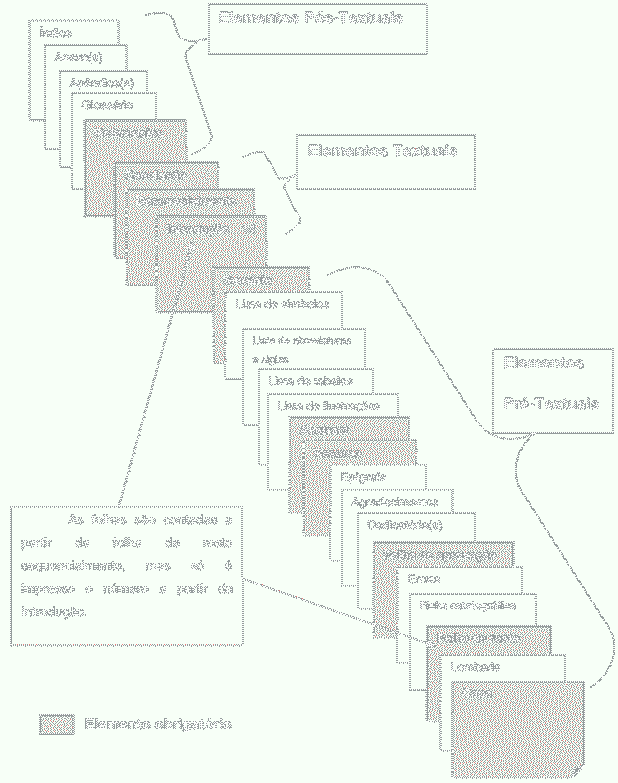
\includegraphics[scale=0.6]{imagens/Estrutura-Trabalhos.png} 
	\newline \footnotesize \textbf{Fonte}: \cite{webLink}.
	\label{fig:EstruturaTrab}
\end{figure}

\section{TEMÁTICA DO TCC}\label{sec:TEMÁTICATCC}
Os temas tratados no TCC devem estar relacionados ao objeto de estudo da Ciência da Computação e estar inseridos em suas subáreas (Quadro 2) e abordar um problema do mundo real, a fim de propor soluções e melhorias. O TCC deve relacionar conhecimentos adquiridos em várias das disciplinas cursadas. Por exemplo, podem envolver algumas das seguintes áreas: inteligência artificial, redes, robótica, pesquisa operacional, grafos, arquitetura de \textit{hardware}, paradigmas de linguagens de programação, comunicação de dados, computação gráfica, matemática/estatística.  

\begin{table}[t]
	\caption{Áreas que compõem a Ciência da Computação de acordo com o CNPQ.}
	\label{tab:AreasCNPQ}
	\begin{tabular}{|l|l|}
		\hline
		\textbf{10300007} & \textbf{CIÊNCIA DA COMPUTAÇÃO}                     \\ \hline
		10301003          & TEORIA DA COMPUTAÇÃO                               \\ \hline
		10301011          & COMPUTABILIDADE E MODELOS DE COMPUTAÇÃO            \\ \hline
		10301020          & LINGUAGEM FORMAIS E AUTÔMATOS                      \\ \hline
		10301038          & ANÁLISE DE ALGORITMOS E COMPLEXIDADE DE COMPUTAÇÃO \\ \hline
		10301046          & LÓGICAS E SEMÂNTICA DE PROGRAMAS                   \\ \hline
		10302000          & MATEMÁTICA DA COMPUTAÇÃO                           \\ \hline
		10302018          & MATEMÁTICA SIMBÓLICA                               \\ \hline
		10302026          & MODELOS ANALÍTICOS E DE SIMULAÇÃO                  \\ \hline
		10303006          & METODOLOGIA E TÉCNICAS DA COMPUTAÇÃO               \\ \hline
		10303014          & LINGUAGENS DE PROGRAMAÇÃO                          \\ \hline
		10303022          & ENGENHARIA DE SOFTWARE                             \\ \hline
		10303030          & BANCO DE DADOS                                     \\ \hline
		10303049          & SISTEMAS DE INFORMAÇÃO                             \\ \hline
		10303057          & PROCESSAMENTO GRÁFICO (GRAPHICS)                   \\ \hline
		10304002          & SISTEMA DE COMPUTAÇÃO                              \\ \hline
		10304010          & HARDWARE                                           \\ \hline
		10304029          & ARQUITETURA DE SISTEMAS DE COMPUTAÇÃO              \\ \hline
		10304037          & SOFTWARE BÁSICO                                    \\ \hline
		10304045          & TELEINFORMÁTICA                                    \\ \hline
	\end{tabular}
	\newline \footnotesize \textbf{Fonte: \cite{Capes2018}.}
\end{table}

\section{SUGESTÕES DE FORMATOS DE TCC}\label{sec:SUGESTOESTCC}
Os TCCs do curso de Bacharelado em Ciência da Computação podem tratar de desenvolvimento de \textit{softwares} comerciais; desenvolvimento de \textit{softwares} científicos; desenvolvimento de \textit{softwares} educacionais; desenvolvimento de metodologias; revisão bibliográfica; e TCC empresa.[não limitar, modalizar]

\subsection{TCC de Desenvolvimento de Software}\label{sec:DesenvolvimentoSof}

Trabalho de conclusão de curso que apresenta o desenvolvimento de um software, desde seu planejamento até o teste prático. Segundo \textcite{Pressman2011}, o software pode ser comercial ou de aplicação, ou seja, um programa sob medida que soluciona uma necessidade específica de negócio, então, é desenvolvido com a finalidade de ser comercializado ou com interesses empresariais. As aplicações nessa área processam dados comerciais ou técnicos de uma forma que facilite as operações comerciais e as tomadas de decisões técnico-administrativas. Ainda, o software desenvolvido pode ser científico ou de engenharia, ou seja, um software que auxilia as aplicações científicas e é geralmente caracterizado por algoritmos de processamento de números. 

Por fim, há o desenvolvimento de software embutido ou embarcado. Trata-se de software próprio para um determinado hardware. O software embutido é usado para controlar produtos e sistemas para os mercados industriais e de consumo, e pode executar funções limitadas e específicas (por exemplo, controle do painel para fornos de micro-ondas) ou oferecer recursos funcionais significativos e capacidade de controle (por exemplo, funções digitais em automóveis, tal como controle de combustível, sistemas de freio) \cite{Pressman2011}. Nesse caso, o TCC pode ter como objetivo produzir tanto o \textit{software} como o hardware.

\subsection{TCC de Análise e Desenvolvimento de Metodologia}\label{sec:AnaliseDese}
O TCC de desenvolvimento de metodologia refere-se à proposta de alternativas ao modelos tradicionais de desenvolvimento de software, [metodologias de redes]. As metodologias devem acelerar a construção de soluções tecnológicas e têm por objetivo a melhoria contínua dos processos, trazendo avanços de comunicação e interação entre a equipe e os usuários, mais organização para o alcance de metas, diminuição de erros e retrabalhos, mais colaboração e, sobretudo, respostas rápidas às mudanças. Tudo isso favorece a geração de mais produtividade para os desenvolvedores, além de redução de custos e até mais satisfação com o trabalho. Novas maneiras de administrar as equipes de TI em projetos de desenvolvimento de software são geradas em função das metodologias ágeis, por exemplo, fazendo com que os usuários sejam participantes na construção das soluções \cite{Sommerville2011}. 

\subsection{TCC de Revisão Bibliográfica}\label{sec:RevisaoBib}
Conforme esclarece \cite{Boccato2006},  a pesquisa bibliográfica busca a resolução de um problema (hipótese) por meio de referenciais teóricos publicados. Analisa e discute as várias contribuições científicas existentes na área de estudo. Esse tipo de pesquisa traz subsídios para o conhecimento sobre o que foi pesquisado, como e sob que enfoque e perspectivas foi tratado o assunto apresentado na literatura científica. Para tanto, é de suma importância que o pesquisador realize um planejamento sistemático do processo de pesquisa, que compreenda desde a definição temática, passando pela construção lógica do trabalho até a decisão de sua forma de comunicação e divulgação.

Assim, um TCC de revisão bibliográfica resgata o estado da arte na área de estudo escolhida e traz conclusões baseadas na análise da literatura revisada.

\subsection{TCC Empresa}\label{sec:Empresa}
Envolve a criação de um produto e sua comercialização, com plano de negócio. É válido somente para empresas pré-encubadas na UTFPR-SH. Embora uma empresa geralmente tenha sócios, o TCC Empresa deve ser individual como os demais TCCs

\subsection{Ilustrações}\label{sec:Ilustracoes}
As ilustrações são um apoio para ajudar no esclarecimento do texto, de modo que apenas ilustrações pertinentes devem ser usadas. Todas elas devem obrigatoriamente estar citadas no corpo do texto, antes de aparecerem. 
Se o produto a ser desenvolvido for um software, o diagrama de casos de uso geral (Figura \ref{fig:CasoDeUso}) deve constar na seção de metodologia, assim como os diagramas de atividade (Figura \ref{fig:Atividades}). Trechos de código, que também entram como figura, devem ser apresentados em pseudocódigo. Diagramas de classes, se houver necessidade de inclusão, devem constar como apêndice. Anexos e apêndices também devem estar referenciados no texto. 

\begin{figure}[htb]
	\centering
	\caption{Exemplo de diagrama de caso de uso geral.}
	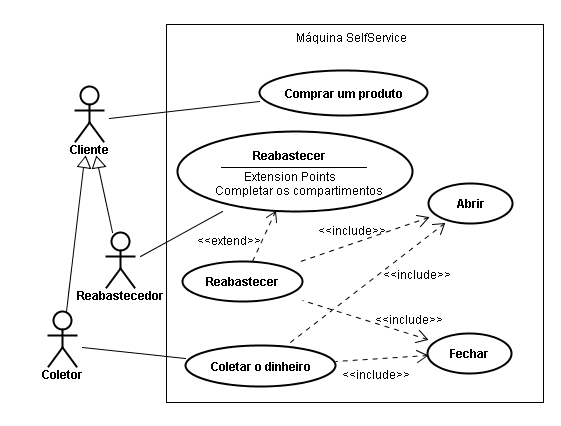
\includegraphics[scale=0.6]{imagens/DiagramaCasoDeUso.png} 
	\newline \footnotesize \textbf{Fonte}: (Própria, 2021).
	\label{fig:CasoDeUso}
\end{figure}

\begin{figure}[htb]
	\centering
	\caption{Exemplo de diagrama de atividade.}
	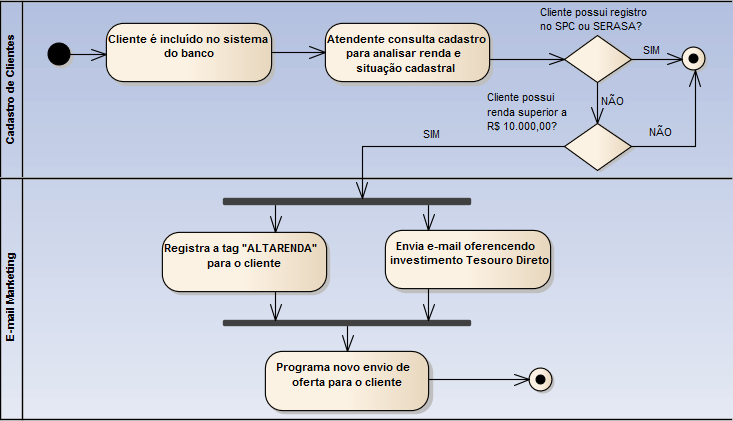
\includegraphics[scale=0.6]{imagens/DiagramaAtividades.png} 
	\newline \footnotesize \textbf{Fonte}: \cite{Ventura2018}.
	\label{fig:Atividades}
\end{figure}

\chapter{ANÁLISE DE RESULTADOS }\label{chp:AnaliseResultados}

Esta seção primária pode se chamar Análise dos Resultados, Resultados, Resultados e Discussão, a critério do autor. Nela, detalhadamente, descrevem-se e discutem-se os resultados do trabalho e seus impactos sociais, ambientais, tecnológicos. No desenvolvimento pode haver outras seções primárias, a depender do tipo de TCC e da metodologia adotada. Por exemplo, pode-se criar Resultados e outra seção chamada Discussão. 

Os resultados referem-se ao que realmente aconteceu no trabalho, não a que o autor gostaria de que acontecesse. Apenas resultados reais, positivos ou negativos, ajudam a impulsionar a ciência, pois são o relato de uma experiência que auxilia e enriquece estudos posteriores.

\pagebreak

%%%%%%%%%%%%%%%%%%%%%%%%%%%%%%%%%%%%%%%%%%%%%%%%%%%%%%%%%%%%
% B I B L I O G R A F I A
%%%%%%%%%%%%%%%%%%%%%%%%%%%%%%%%%%%%%%%%%%%%%%%%%%%%%%%%%%%%
% Retirar esta parte se o trabalho não tiver bibliografia
\printbibliography
\newpage


%%%%%%%%%%%%%%%%%%%%%%%%%%%%%%%%%%%%%%%%%%%%%%%%%%%%%%%%%%%%
% G L O S S A R I O (opcional, remova o comentário caso queira utilizar)
%%%%%%%%%%%%%%%%%%%%%%%%%%%%%%%%%%%%%%%%%%%%%%%%%%%%%%%%%%%%
%\makeglossarypage{\item [Palavra] Significado da palavra

\item [Palavra 2] Significado da palavra 2

}

%%%%%%%%%%%%%%%%%%%%%%%%%%%%%%%%%%%%%%%%%%%%%%%%%%%%%%%%%%%%
% A N E X O (opcional)
%%%%%%%%%%%%%%%%%%%%%%%%%%%%%%%%%%%%%%%%%%%%%%%%%%%%%%%%%%%%
\annex
\annexchapter{A}{EXEMPLOS DE OBJETIVO GERAL E ESPECÍFICOS}

                 

Exemplo 2 \\



\begin{mdframed}
	
1.1 OBJETIVO GERAL

O objetivo deste trabalho é modelar, analisar e simular processos de workflow utilizando redes de Petri contínuas com base na ferramenta MATLAB Petri net Toolbox. 

1.1.1 Objetivos Específicos

1)	Mostrar os procedimentos para produzir modelos baseados em redes de Petri contínuas para representar processos de workflow; 

2)	Elaborar um estudo comparativo entre os resultados das simulações do modelo discreto e do modelo contínuo. \linebreak

\end{mdframed}


Exemplo 3  \\



\begin{mdframed}
	
1.1 OBJETIVO GERAL

Aplicar ferramentas otimizadas de visão computacional e aprendizado de máquina supervisionado para verificar o desempenho de algoritmos computacionais de reconhecimento facial e indicar sua viabilidade no desenvolvimento de ferramentas de controle de acesso de indivíduos, a fim de avaliar a robustez de cada algoritmo, usando um conjunto de 3 bancos de dados: Yale, ORL e outro criado com a junção dos dois bancos anteriormente citados.

1.1.1 Objetivos Específicos
\begin{enumerate}
	\item Levantar as principais abordagens de reconhecimento facial e estratégias de cada algoritmo; 
	
	\item Identificar as contribuições e limitações de cada método em diferentes ambientes e tipos de imagem, classificando os algoritmos e técnicas por eficiência e uso;
	
	\item Elaborar um estudo comparativo dos algoritmos com diferentes bancos de imagens, analisando os aspectos intrínsecos da imagem na distorção de cada método;
	
	\item Elaborar uma rotina de experimentos e visualizar os resultados com separação de algoritmos e bases para justificar a indicação de uso de cada método pelo tipo de imagem especializada.\linebreak
	
\end{enumerate}

\end{mdframed}




\end{document}
